\documentclass[12pt,a4paper]{article}

\usepackage[utf8]{inputenc}
\usepackage{lmodern}
\usepackage[T1]{fontenc}
% paysage
% \usepackage[landscape]{geometry}
\usepackage{lscape}
\usepackage{graphicx}
% \graphicspath{ {images/} }

% headers footers
\usepackage{fancyhdr}
\pagestyle{fancy}

% référencer la dernière page
\usepackage{lastpage}

% pdf
\usepackage{pdfpages}

% math
\usepackage{amssymb}

\usepackage{multicol}
\usepackage{url}

\usepackage{multido}
\usepackage[utf8]{inputenc}
% \usepackage{lmodern}
\usepackage[T1]{fontenc}

\usepackage[sfdefault]{AlegreyaSans} %% Option 'black' gives heavier bold face
%% The 'sfdefault' option to make the base font sans serif
% \renewcommand*\oldstylenums[1]{{\AlegreyaSansOsF #1}}


\usepackage{multicol}
\usepackage[frenchb]{babel}
% \usepackage{pstricks,pst-plot,pst-node}
% \usepackage{pstricks-add}
\usepackage{pst-circ}
\usepackage{pst-magneticfield}
\usepackage{pst-electricfield}
\usepackage{graphicx}
\usepackage{amsmath,amsfonts,amssymb}
\usepackage{titlesec} 
\usepackage{float}
\usepackage{textcomp}
\usepackage{amssymb}
\usepackage[toc,page]{appendix}
\usepackage{listings} 

\lstset{language=Matlab}
\usepackage{lipsum}
\usepackage{enumerate}


%Numerotation par section des équations
\usepackage{amsmath}

\usepackage{tabularx}
\usepackage{longtable}

%------------------------------inclue les références
% \usepackage[nottoc, notlof, notlot]{tocbibind}
%\usepackage{biblatex}
% \usepackage{csquotes}

%\usepackage{etoolbox}
% \patchcmd{\chapter}{\thispagestyle{plain}}{\thispagestyle{fancy}}{}{}
\title{
	\Huge\textsc{Quadrilatère articulé\\
		Mécanisme à quatre barres}
}
\author{Mohamed Thebti} 

\begin{document}
% retrait de la première ligne d'un paragraphe
\setlength{\parindent}{0mm}

\fancyhead[R]{\slshape \leftmark}
\fancyhead[L]{\slshape Mécanisme à quatre barres}
%\fancyhead[LE,RO]{\slshape \rightmark}
% \fancyhead[LO,RE]{\slshape \leftmark}

% \fancyfoot[C]{Travail de Master}
\fancyfoot[L]{\slshape Thebti Mohamed}
\fancyfoot[C]{}
\fancyfoot[R]{\thepage}

\maketitle
\newpage

\tableofcontents

\newpage



\section{Introduction}

Le quadrilatère articulé est un mécanisme qui se trouve dans beaucoup d'applications.
\medbreak
Dans ce document, il s'agit de présenter des exemples de quadrilatère articulé et les méthodes mathématiques permettant de

\begin{itemize}
	\item faire une étude cinématique
	\item établir les équations de mouvement
	\item et résoudre ces équations
\end{itemize}



\section{Définition d'un quadrilatère articulé}


Il s'agit d'un mécanisme formé de quatre quatre barres reliées entre elles par des liaisons pivots. Dans la littéreatue, il est aussi appelé "mécanisme à 4 barres".

\medbreak
Ce mécansisme se trouve dans plusieurs applications, comme le cric d'une voiture, le système d'ouverture d'une barrière ou le mouvement du bras d'une pelle mécanique (qui se résume à plusieurs quadrilatères articulés assemblés ensemble). 
\medbreak
. 
\medbreak
L'objectif de ce document est de présenter une étude cinématique afin de prévoir le mouvement de ce mécanisme. Les méthodes mathématiques seront exposées et des exemples pratiques concluront le document. 

\medbreak
Cette étude a aussi pour but d'avoir les outils nécessaire afin d'engager une étude dynamique plus complexe de type de mécanisme. 

\subsection{Quelques exemples}
mettre photo : \\
cric voiture, bras pelle mécanique, système automatique de barrière, 
\section{Étude cinématique}

\subsection{Schéma du mécanisme}
(mettre le schéma ici)
une des barre est fixée et assimililée au bâti. Ainsi, ici c'est le bras $OC$.\\

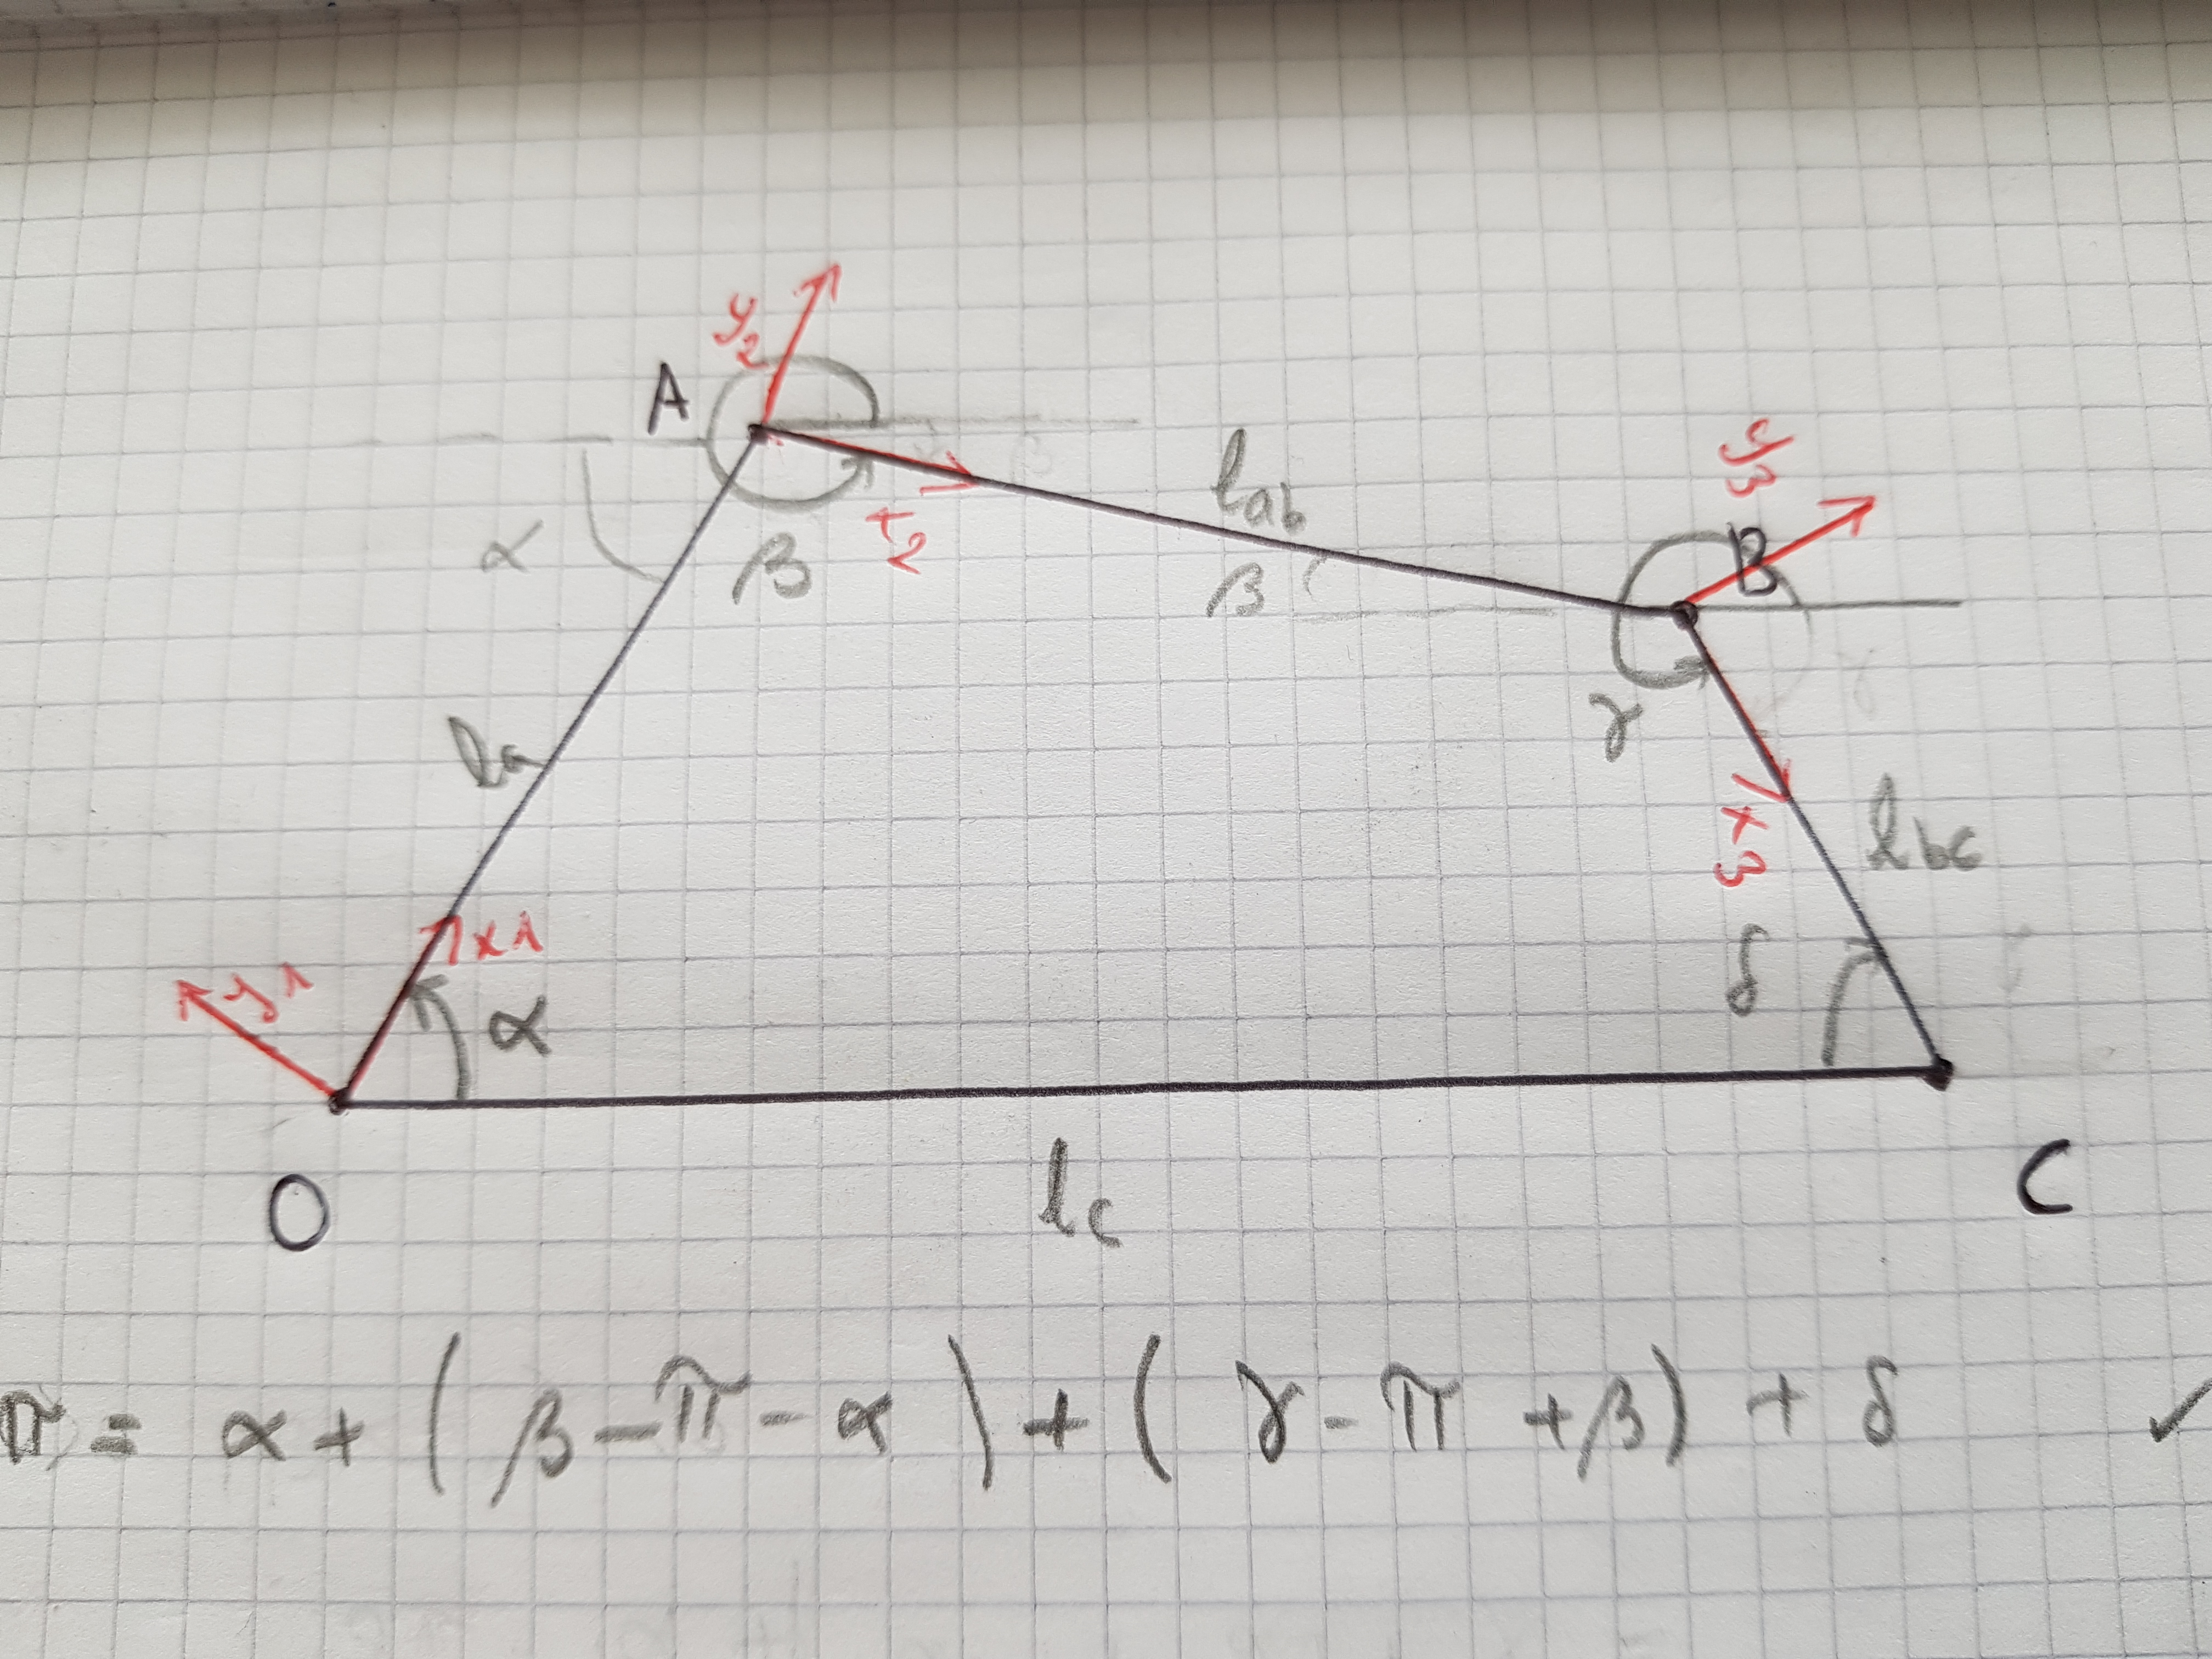
\includegraphics[scale=0.1]{schema.png}
\subsection{Variables et degré de liberté}
Ce système possède huit  variables :
\begin{itemize}
	\item Quatre angles : $\alpha$, $\beta$, $\gamma$, $\delta$\\
Ces angles sont inter-intdépendants avec la relation suivante : 
\begin{equation}
2 \pi = \alpha + (\beta - \pi - \alpha) + (\gamma - \pi - \beta)+ \delta
\end{equation}
L'angle $\delta$ est négligé car il est est exprimé par $\delta = 2\pi - \gamma$
	\item Quatre longueurs de bras : $l_a$,$l_{ab}$,$l_{bc}$ et $l_c$\\
\end{itemize}
Au final, le système a sept variables.
Calcul du nombre de ddl : (relations)....\\
Nombre de ddl : 1\\

pour commander ce type de mécanisme, on commande une variable et on fixe les 6 autres. 



\subsection{Repère global}

Il est placé à l'origine $O$, qui est un point fixe. Le repère global $R$ est utilisé pour exprimer la position des point $A$, $B$ et $C$ durant le mouvement du quadrilatère.
\begin{equation}
R=\{x,y,z\}
\end{equation}
\medbreak
\medbreak

\begin{figure}[H]
	\centering
%	\includegraphics[scale=2]{Vue_dessus.png}
	\caption{Vue de dessus}
\end{figure}

\subsection{Matrice de rotation et repères locaux}

Le quadrilatère se déplace dans le plan $XZ$, et la résolution du mécanisme se fait dans ce plan. les repères locaux sont définis par une rotation selon l'axe $Y$ du repère global $R$.\\

La matrice de rotation d'un angle quelconque $\alpha$ selon l'axe $Y$ est la suivante : 
\begin{equation}
Rot_Y(\alpha)=Rot(\alpha)=
\begin{bmatrix}
cos(\alpha) & 0 &-sin(\alpha)\\
0 & 1 & 0 \\
sin(\alpha) & 0 & cos(\alpha) \\
\end{bmatrix}
\end{equation}
selon la figure ...., les repères locaux sont définis de la manière suivante : 
ce sont des repères mobiles, qui bougent avec les bras sur lesquels ils sont placés. Ainsi chacun dépend du repère précédent : le repère $R_{i+1}$ se déplacent selon un axe du repère $R_i$.
\medbreak

\begin{itemize}
	\item Repère 1 : placé en $O$, rotation de $\alpha$ autour de l'axe $Y$.
\begin{equation}
R_1=\{x_1,y_1,z_1\}
\end{equation}
	\item Repère 2 : placé en $A$, rotation de $\beta$ autour de l'axe $Y$.
\begin{equation}
R_2=\{x_2,y_2,z_2\}
\end{equation}
	\item Repère 3 : placé en $B$, rotation de $\gamma$ autour de l'axe $Y$.
\begin{equation}
R_3=\{x_3,y_3,z_3\}
\end{equation}
	\item Repère 4 : placé en $C$, rotation de $\delta$ autour de l'axe $Y$.
\begin{equation}
R_4=\{x_4,y_4,z_4\}
\end{equation}
\end{itemize}




\medbreak



\medbreak


\subsection{Passage d'un repère à un autre}
Matrice de transformation $T_i$ du repère $i+1$ à $i$ : 
\begin{equation}
\vec{A}_{R_i{i+1}}=T_i \cdot \vec{A}_{R_i}
\end{equation}

Pour la suite, nous avons besoin d'exprimer la position d'un point par rapport au repère global. En partant de la relation précédente, on peut en déduire : 
\begin{equation}
\vec{A}_R=T_1 \cdot T_2 \cdot .... \cdot T_i \cdot \vec{A}_{R_i}
\end{equation}


\subsection{Les vecteurs de position}

définir les vecteurs qui expriment les barres de la pelle mécanique, selon les repères définis précédemment. 

\begin{equation}
\vec{OA}_{R_1}=
\begin{bmatrix}
oa \\
0\\
0
\end{bmatrix}_{R_1} \enspace
\vec{AB}_{R_{2}}=
\begin{bmatrix}
ab \\
0\\
0
\end{bmatrix}_{R_2} \enspace
\vec{BC}_{R_{3}}=
\begin{bmatrix}
bc \\
0\\
0
\end{bmatrix}_{R_3} \enspace
\vec{OC}_{R_4}=
\begin{bmatrix}
co \\
0\\
0
\end{bmatrix}_{R}
\end{equation}

\medbreak

\subsection{Positions des pivots exprimées dans le repère global}
\begin{eqnarray}
\vec{OA}_R=Rot(\alpha) \cdot \vec{OA}_{R_1}=
\begin{bmatrix}
cos(\alpha) & 0 &-sin(\alpha)\\
0 & 1 & 0 \\
sin(\alpha) & 0 & cos(\alpha) \\
\end{bmatrix}
\begin{bmatrix}
oa \\
0\\
0
\end{bmatrix}_{R_1} =
\begin{bmatrix}
oa \cdot cos(\alpha) \\
0\\
oa \cdot sin(\alpha) 
\end{bmatrix}_{R}
\\
\vec{AB}_R=Rot(\beta) \cdot \vec{AB}_{R_2}=
\begin{bmatrix}
cos(\beta) & 0 &-sin(\beta)\\
0 & 1 & 0 \\
sin(\beta) & 0 & cos(\beta) \\
\end{bmatrix}
\begin{bmatrix}
ab \\
0\\
0
\end{bmatrix}_{R_2}=
\begin{bmatrix}
ab \cdot cos(\beta) \\
0\\
ab \cdot sin(\beta) 
\end{bmatrix}_{R}
\\
\vec{BC}_R =Rot(\gamma) \cdot \vec{ BC}_{R_3}=
\begin{bmatrix}
cos(\gamma) & 0 &-sin(\gamma)\\
0 & 1 & 0 \\
sin(\gamma) & 0 & cos(\gamma) \\
\end{bmatrix}
\begin{bmatrix}
bc \\
0\\
0
\end{bmatrix}_{R_3}=
\begin{bmatrix}
bc \cdot cos(\gamma) \\
0\\
bc \cdot sin(\gamma) 
\end{bmatrix}_{R}
\\
\vec{OC}_R = Rot(\delta) \cdot \vec{OC}_{R_4}=
\begin{bmatrix}
cos(\delta) & 0 &-sin(\delta)\\
0 & 1 & 0 \\
sin(\delta) & 0 & cos(\delta) \\
\end{bmatrix}
\begin{bmatrix}
oc \\
0 \\
0
\end{bmatrix}_{R} =
\begin{bmatrix}
oc \cdot cos(\delta) \\
0\\
oc \cdot sin(\delta) 
\end{bmatrix}_{R}
\end{eqnarray}
Une fois que le système est résolu, il est possible de connaître la position de chaque articulation du mécanisme grâce aux relations suivantes :
\begin{eqnarray}
\vec{OA}_R=
\begin{bmatrix}
oa \cdot cos(\alpha) \\
0\\
oa \cdot sin(\alpha) 
\end{bmatrix}_{R}
\\
\vec{OB}_R=\vec{OA}_R+\vec{AB}_R=
\begin{bmatrix}
oa \cdot cos(\alpha) +ab \cdot cos(\beta)\\
0\\
oa \cdot sin(\alpha) + ab \cdot sin(\beta)
\end{bmatrix}_{R}\\
\vec{OC}_R=\vec{OA}_R+\vec{AB}_R+\vec{ BC}_R =
\begin{bmatrix}
oa \cdot cos(\alpha) +ab \cdot cos(\beta)+bc \cdot cos(\gamma)\\
0\\
oa \cdot sin(\alpha) + ab \cdot sin(\beta)+bc \cdot sin(\gamma) 
\end{bmatrix}_{R} \\
\vec{OC}_R=
\begin{bmatrix}
oc \cdot cos(\delta) \\
0\\
oc \cdot sin(\delta) 
\end{bmatrix}_{R}
\end{eqnarray}
\newpage
\section{Résolution}
\subsection{Boucle vectorielle fermée}
Départ en $O$, on fait le tour. évidemment, la fonction est nulle, normalement. on résoud ce système d'équation pour minimiser la fonction fonction $\vec{\Phi}$ et atteindre $\vec{\Phi}=\vec{0}$.
\begin{eqnarray}
\vec{\Phi}=\vec{0}=\vec{OA}_R + \vec{AB}_R + \vec{BC}_R - \vec{OC}_R\\
\vec{\Phi}=
\begin{bmatrix}
\Phi_1\\
\Phi_2\\
\Phi_3
\end{bmatrix}=
\begin{bmatrix}
oa \cdot cos(\alpha) +ab \cdot cos(\beta)+bc \cdot cos(\gamma)-oc \cdot cos(\delta)\\
0\\
oa \cdot sin(\alpha) + ab \cdot sin(\beta)+bc \cdot sin(\gamma)-oc \cdot sin(\delta)  
\end{bmatrix}_{R}
\end{eqnarray}

\subsection{Choix de la variable pilotée}
Pour résoudre ce système, quatre variables sont fixées et une variable $q_1$est pilotée.
Il y a deux approches pour contrôler le mouvement du quadrilatère articulé : 
\begin{itemize}
	\item Approche A : piloter un angle. Exemple : quadrilatère de direction de véhicule. (photo)
	\item Approche B : piloter la longueur de bras. Exemple, mouvement du bras d'une pelle mécanique à travers des vérins. (photo)
\end{itemize}
Il reste donc deux inconnues à déterminer. On définit $\vec{q}$ le vecteur qui les contient :
\begin{equation}
\vec{q}=\begin{bmatrix}
q_2\\
q_3
\end{bmatrix}
\end{equation}


\subsection{Méthode de Newton-Raphson}
Résoudre le système $\vec{\Phi}$ revient à chercher la combinaison de $\alpha$, $\beta$ et $\gamma$ qui satisfait la condition $\vec{\Phi}=\vec{0}$.

La méthode à utiliser est celle de Newton-Raphson (fonction à plusieurs variables $\vec{\Phi}(x,y,...)$), adaptée à partir de la méthode de Newton (fonction à une variable $\Phi(x)$).

\subsubsection{Méthode de Newton}
on cherche le zéro d'une fonction : $\Phi(x)=0$. 
Méthode de la tangente : 
\begin{eqnarray}
0 = f(x_i) + f'(x_i) (x_{i+1}-x_i)\\
\Delta x = (x_{i+1}-x_i) = -\frac{f(x_i)}{f'(x_i)}\\
x_{i+1}=x_i -\frac{f(x_i)}{f'(x_i)}
\end{eqnarray}

Pour que la méthode converge, il faut que le point de départ des itérations soit assez proche du vrai zéro. En pratique, une simple étude de fonction permet de situer le zéro cherché. Ensuite, la valeur de départ est choisie assez proche de ce zéro. 

\subsection{Application de la méthode de Newton-Raphson}
Pour passer de 1D à plusieurs dimensions, la conversion suivante est appliquée : 
\begin{eqnarray}
x_{i+1} \rightarrow \vec{q}_{i+1}\\
x_{i} \rightarrow \vec{q}_{i}=\begin{bmatrix}
q_{1_i} \\
q_{2_i} 
\end{bmatrix}\\
f(x_i) \rightarrow \vec{\Phi}(\vec{q}_{i})=\begin{bmatrix}
\Phi_{1}(\vec{q}_{i}) \\
\Phi_{2}(\vec{q}_{i}) 
\end{bmatrix}\\
f'(x_i) \rightarrow J(\vec{q}_{i})
\end{eqnarray}
Le jacobien $J(\vec{q}_{i})$ est défini par les dérivées partielles de la fonction $\vec{\Phi}$ par rapport aux inconnues $q_1$ et $q_2$ : 
\begin{eqnarray}
J=
\begin{bmatrix}
\frac{\delta \Phi_1}{\delta q_2} & \frac{\delta \Phi_1}{\delta q_3}\\
\frac{\delta \Phi_2}{\delta q_2} & \frac{\delta \Phi_2}{\delta q_3}
\end{bmatrix}
\end{eqnarray}
Ainsi, résoudre ce système de plusieurs équations se fait de la manière suivante : 
\begin{eqnarray}
\vec{0} = \vec{\Phi}(\vec{q}_i) + J(\vec{q}_i) (\vec{q}_{i+1}-\vec{q}_i)\\
\Delta \vec{q} = \vec{q}_{i+1}-\vec{q}_i =  -J^{-1}(\vec{q}_i) \cdot \vec{\Phi}(\vec{q}_i)\\
\vec{q}_{i+1}=\vec{q}_{i}-J^{-1}(\vec{q}_i) \cdot \vec{\Phi}(\vec{q}_i)
\end{eqnarray}

\subsection{Algorithme d'itération}
L'intervalle de la variable pilotée $q_1$ est connue. Pour chaque valeur, des valeurs de départ pour le vecteur des inconnues sont données, ce qui permet de calculer :
\begin{eqnarray}
\vec{q}_{0}=\begin{bmatrix}
q_{2_0} \\
q_{3_0} 
\end{bmatrix}\\
\vec{\Phi}(\vec{q}_{0})=\begin{bmatrix}
\Phi_{1}(\vec{q}_{0}) \\
\Phi_{2}(\vec{q}_{0}) 
\end{bmatrix}\\
\vec{J}(\vec{q}_{0})\\
\vec{q}_{1}=\vec{q}_{0} - \vec{J}(\vec{q}_{0}) \cdot \vec{\Phi}(\vec{q}_{0})
\end{eqnarray}

Ensuite, il s'agit d'effectuer les itérations suivantes : 
\begin{enumerate}
	\item Calculer $\vec{q}_{i}$
	\item Calculer $\vec{\Phi}(\vec{q}_{i})$
	\item Calculer $J(\vec{q}_{i})$
	\item Calculer l'inverse du jacobien $J^{-1}(\vec{q}_{i})$
	\item Calculer le vecteur $\vec{q}$ suivant avec : 
	\begin{eqnarray}
	\Delta \vec{q} = -J^{-1}(\vec{q}_i) \cdot \vec{\Phi}(\vec{q}_i)\\
	\vec{q}_{i+1}=\Delta \vec{q}+\vec{q}_{i}
	\end{eqnarray}
	\item Stopper les itérations si :
\begin{equation}
\vec{\Phi}(\vec{q}_{i}) < \epsilon
\end{equation}
ou 
\begin{equation}
n_{itération}=max(i)=N_{max}
\end{equation}
\end{enumerate}

Le résultat est un tableau qui donne les valeurs de $q_2$ et $q_3$ selon $q_1$.

\subsection{Situations singulières}
selon les longueurs des bras et des angles, il y a des positions singulières, des positions où le mouvement ne peut plus être déterminées. (exemple de situations singulières), 
Mathématiquement, Méthode de Newton : dérivée nulle. Newton-Raphson : le jacobien n'est pas inversible. 
\medbreak
Quand on dimensionne le système, il faut étudier les situations singulières. Soit on les évite, soit on assure que le système ne s'arrête pas dans ces positions. 
\section{Approche A : exemple pratique}
Les longueurs des quatre barres sont connues. L'angle $\alpha$ est piloté:  \\
Les deux inconnues sont les angles $\beta$ et $\gamma$. On définit $\vec{q}$ le vecteur des inconnues :
\begin{equation}
\vec{q}=\begin{bmatrix}
\beta\\
\gamma
\end{bmatrix}
\end{equation}

valeur numérique : 
$q_1$ : pi/4 à pi/2. \\

graphe $q_2$ et $q_3$ selon $q_1$
\section{Approche B : exemple pratique}
Les longueurs $l_a$, $l_{bc}$ et $l_{c}$ et l'angle $\alpha$ sont connus. La longueur $l_{ab}$ est pilotée : godet pelle mécanique. \\
Les deux inconnues sont les angles $\beta$ et $\gamma$. On définit $\vec{q}$ le vecteur des inconnues :
\begin{equation}
\vec{q}=\begin{bmatrix}
\beta\\
\gamma
\end{bmatrix}
\end{equation}


\section{Mouvement de quelques mécanismes à quatre barre}



\section{Conclusion}
ici, problème plan en deux dimensions.

il est bien sûr possible d'imaginer un mécanisme à quatre barres dans l'espace 3D. dans ce cas, il y aura plus de ddl et donc, plus de variable à pilotés. 

\end{document}